\documentclass[11pt]{article}
\usepackage{fullpage}
\usepackage{amsmath}
\usepackage{pdfpages}
\usepackage{booktabs}

\begin{document}

	\pagenumbering{roman}	
	\pagestyle{empty}
	\title{Praktikumsbericht\\Physik Praktikum\\Versuch: E1\\Elektrische Messtechnik\\}
	\author{Autor: Janosch Ehlers\\Gruppe C2}
	\date{Datum d. Versuchsdurchführung:\\Do, 09.05.2019}
	\maketitle
	\thispagestyle{empty}	
	
	\newpage
	\pagestyle{plain}
	\pagenumbering{arabic}
	\section*{1. Ziel des Experiments}
Dieses Experiment zielt darauf ab, die Grundlagen der Elektrotechnik, wie Reihen- und Parallelschaltung zu untersuchen und anzuwenden. Dabei wird untersucht, wann Stromrichtiges Messen und Spannungsrichtiges messen Sinnvoll ist. Auch werden Wechselspannungen mit verschiedenen Messgeräten gemessen und die Kennlinie einer Leuchtdiode aufgezeichnet.

	\section*{2. Theoretischer Hintergrund}
In jeder elektrischen Schaltung werden mindestens drei physikalische Größen beachtet: die Spannung: $U$, die Stromstärke: $I$ und der Widerstand: $R$. In jeder Schaltung,  welche keinen Kurzschluss erzeugt, ist die Stromstärke abhängig von dem Gesamtwiderstand (auch Last genannt) und der angelegten Spannung. Diese drei Größen sind definiert über:
	\begin{equation}
	U=R\cdot I
	\end{equation}
Nun können weitere Verbraucher in den Stromkreis integriert werden. Jeder Verbraucher, hat einen eigenen Widerstand. Weiterhin wichtig ist, das an jedem Widerstand eine Spannung ($U\textsubscript{d}$) zwischen Ein- und Ausgang gemessen werden kann. Es gilt:
	\begin{equation}
	\sum_{i=1}^{N}U\textsubscript{di}=U\textsubscript{0}
	\end{equation}
Auch ist zu erwähnen, dass an jeder Verzweigung in einem Schaltkreis, die Stromstärke entsprechend der an dem Zweig liegenden Last gespalten wird. Da sich an keinem Knotenpunkt eine Ladung aufbaut, muss folgendes gelten:
	\begin{equation}
	\sum_{j=1}^{N}I\textsubscript{j}=0
	\end{equation}
Gleichung (2) und (3) werden im folgenden auch 1. bzw. 2. Kirchhoff'scher Satz genannt. Betrachtet man nun einen Schaltkreis mit mehreren Widerständen, so können diese entweder in Reihe (siehe Abbildung 1), oder parallel (siehe Abbildung. 2) geschaltet Sein.\\
\begin{center}
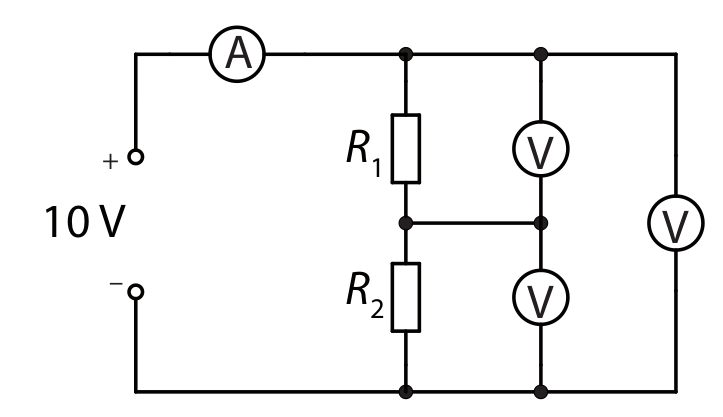
\includegraphics[scale=0.3]{./Reihe.png}\\
\small \textsc{Abbildung 1 - Reihenschaltung von Widerständen}\\
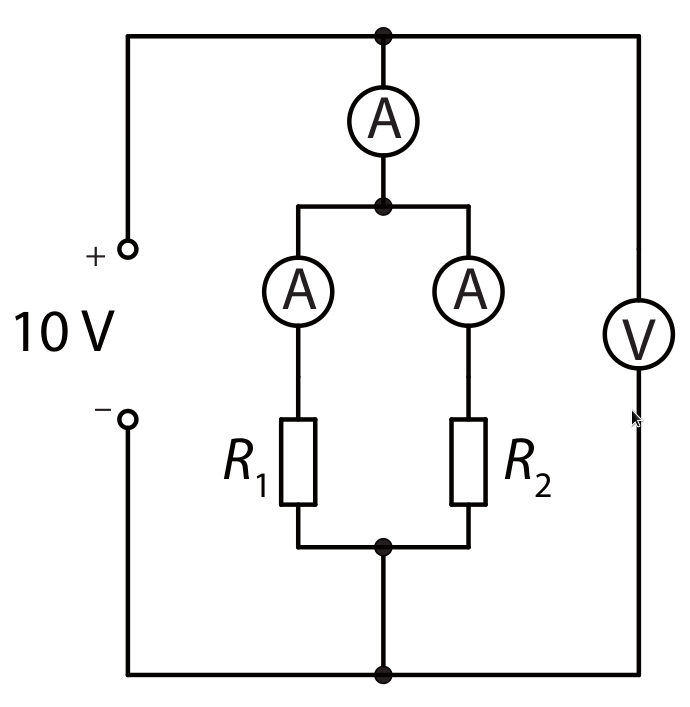
\includegraphics[scale=0.3]{./parallel.png}\\
\small \textsc{Abbildung 2 - Parallelschaltung von Widerständen}\\
\end{center}
In einer Parallelschaltung wird der Strom auf beide Widerstände aufgeteilt, an den einzelnen Widerständen kann allerdings keine Differenz zwischen den Spannungsabfällen gemessen werden. Im zweiten Beispiel werden die Widerstände in Reihe geschaltet. Hier kann an jedem Widerstand der Spannungsabfall gemessen werden. Die Stromstärke bleibt allerdings für die gesamte Reihe konstant. Dies ist über die folgenden Gleichungen definiert:
	\begin{equation}
	U=U\textsubscript{2}\frac{R\textsubscript{2}}{R\textsubscript{1}+R\textsubscript{2}}\\
	\end{equation}
	\begin{equation}	
	U=\sum_{i=1}^{n}R\textsubscript{i}\cdot I\textsubscript{i}
	\end{equation}
Gleichung (4) findet Verwendung in Reihenschaltungen und Gleichung (5) in Parallelschaltungen. Die bisher beschriebenen Systeme beziehen sich auf Gleichstrom (auch DC, "direkt Current" genannt). Hier wird durch die Stromquelle eine gleichbleibende elektrische Spannung auf den Schaltkreis ausgeübt. Eine andere Art und Weise elektrische Spannung zu erzeugen ist über Erzeugung eines Wechselstroms. Hier wird eine schwingende Spannung mit bestimmter Frequenz und Amplitude erzeugt. Je nach Begebenheit werden beide Spannungsarten kombiniert. So kann z. B. ein sogenanntes DC-Offset der Wechselspannung addiert werden. Hier wird lediglich der Wechselspannung eine Gleichspannung addiert. Wechselspannungen können im Allgemeinen über (6) visualisiert werden.	
	\begin{equation}
	U=U\textsubscript{ampl}\cdot \sin(\omega t)+c
	\end{equation}
Hier wird die resultierende Wechselspannung ($U$) über die Amplitude ($U\textsubscript{ampl}$), der Kreisfrequenz der Schwingung ($\omega$) und dem DC-Offset ($c$), als Funktion der Zeit ($t$) definiert. Die Amplitude einer Wechselspannung ist allerdings nicht zu verwechseln mit dem Spitze-Spitze Wert ($U\textsubscript{SS}$) einer Schwingung. Dieser ist über $U\textsubscript{SS}=2\cdot U\textsubscript{ampl}$ definiert. Weiterhin wichtig ist der Effektiv-Wert($U\textsubscript{eff}$) einer Wechselspannung. Dies ist der Wert, der gemessen wird bei einer AC-Spannungsmessung mit einem Multimeter. Definiert ist dieser über (7).
	\begin{equation}
	U\textsubscript{eff}=\frac{1}{\sqrt{2}}\cdot u\textsubscript{ampl}
	\end{equation}
Beim gleichzeitigen Messen von zwei elektrischen Größen ist zwischen zwei Messungen zu unterscheiden: Der Stromrichtigen und der spannungsrichtigen Messung. Da jedes Messgerät einen eigenen Widerstand hat. Zweck ist das Ausschließen eines Fehlers, der durch den Widerstand der Messgeräte verursacht wird. Den Aufbau einer Stromrichtigen Messung ist in Abbildung 3 Dargestellt, während Abbildung 4 den Aufbau einer spannungsrichtigen Messung darstellt. Effektiv wird in einer stromrichtigen Messung ein Aufbau gewählt, bei der das Voltmeter parallel zum Ampermeter und dem zu Messenden Widerstand, welche in Reihe stehen, geschaltet ist. Bei einer spannungsrichtigen Messung wird das Voltmeter nur parallel zu dem zu Messenden Widerstand geschaltet und nicht parallel zu dem Amperemeter, dieses muss allerdings in Reihe mit der Widerstand-Voltmeter Parallelschaltung stehen.\\
\begin{center}
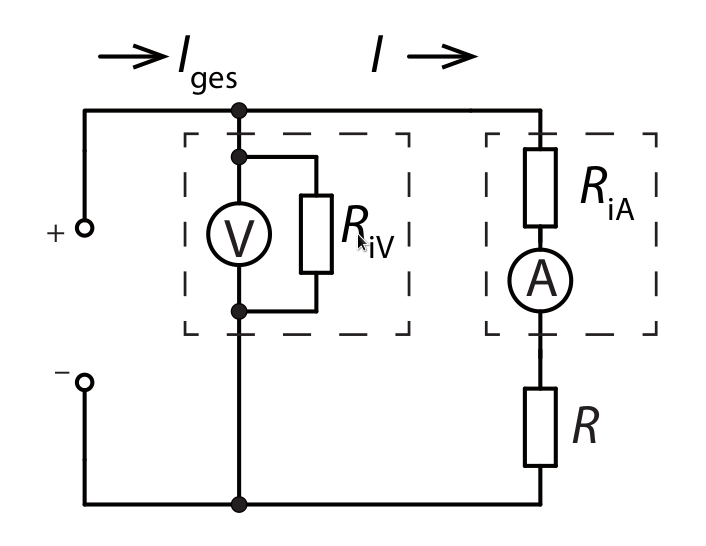
\includegraphics[scale=0.3]{./Stromrichtig.png}\\
\small \textsc{Abbildung 3 - Stromrichtige Messung}\\
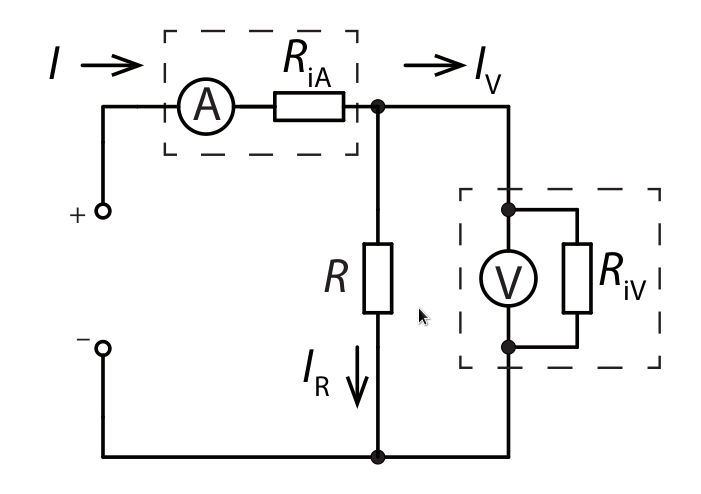
\includegraphics[scale=0.3]{./Spannungsrichtig.png}\\
\small \textsc{Abbildung 4 - Spannungsrichtige Messung}\\
\end{center}

\section*{3. Versuchsaufbau und -durchführung}
Allgemein wurden hier folgende Geräte verwendet: Spannungsversorgungsgerät, Steckbrett, mehrere unterschiedliche Analog- und Digitalmultimeter, ein Zwei-Kanal-Oszilloskop und ein Funktionsgenerator (Siehe Skript). Dabei wurde in einem ersten Aufbau nach Abbildung 1 Zwei Widerstände spannungsrichtig in Reihe gemessen. Dabei wurden folgende Widerstände verwendet: $R_1=1\textrm{k}\Omega$ und $R_2=1\textrm{k}\Omega$ in einem zweiten Durchlauf wurden dann folgende Widerstände verwendet: $R_1=1\textrm{k}\Omega$ und $R_2=10\textrm{k}\Omega$ Danach wurden in einem zweiten Aufbau nach Abbildung 2 Die gleichen Paarungen an Widerständen stromrichtig vermessen. Als Nächstes wurde eine Schaltung nach Abbildung 3 und Abbildung 4 aufgebaut. Nun soll hier die Größe von Widerständen berechnet werden, welche als 0,7 - 1,5 $\Omega$, 100 $\Omega$, 100 $\textrm{k}\Omega$, 20 $\textrm{M}\Omega$ gekennzeichnet sind. Das Spannungsversorgungsgerät wurde dabei auf 10 V mit einer Strombegrenzung von 100 mA eingestellt. 
Anschließend wurde die in Abbildung 5 dargestellte Schaltung aufgebaut. Hier wurde untersucht, bei welchen Frequenzen das Voltmeter den richtigen Effektivwert anzeigt. 
\begin{center}
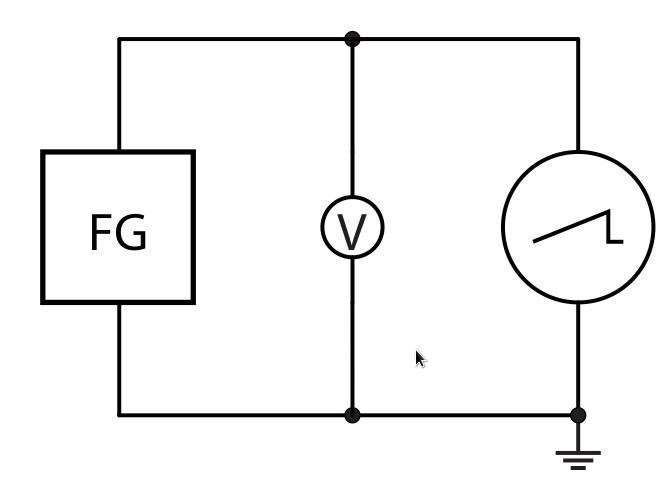
\includegraphics[scale=0.3]{./nr4.png}\\
\small \textsc{Abbildung 5 - Messung von Wechselspannungen mit einem Voltmeter}\\
\end{center}
Dabei wurden 5 beliebige Frequenzen zwischen 1 Hz und 20 kHz untersucht. Der Frequenzgenerator wurde dabei auf einen Spitze-Spitze-Wert von 5 V einem DC-Offset von 0 V eingestellt. Bei dem nächsten Versuch wurde der Aufbau beibehalten, allerdings wurde der Frequenzgenerator auf 65 Hz und einem DC-Offset von 4 V eingestellt. Hier wurde nun das Verhalten des Multimeters in seiner DC-Messeinstellung und seiner AC-Messeinstellung untersucht. In einem letzten Versuchsaufbau gemäß Abbildung 6, wurde das Verhalten einer 5 Hz Schwingung mit einem DC-Offset von 0 V und einem Spitz-Spitze Wert von 10 V in der oben genannten Schaltung untersucht. 
\begin{center}
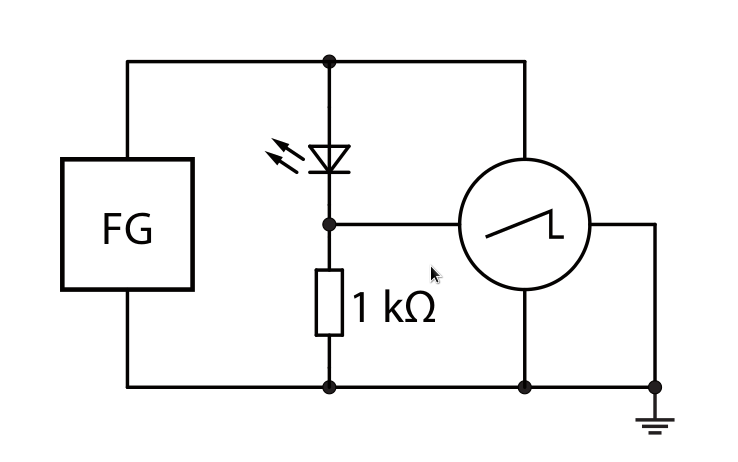
\includegraphics[scale=0.3]{./nr5.png}\\
\small \textsc{Abbildung 6 - Messung einer Dioden-Widerstands Reihenschaltung mit einem Oszilloskop}\\
\end{center}

\section*{4. Auswertung}
Alle Messwerte des ersten Versuchs, sowohl des Spannungsrichtigen als auch des stromrichtigen Aufbaus, ist der Tabelle 1 im Anhang zu entnehmen. Der Quotient der Widerstände liegt innerhalb des Fehlerbereichs des Quotienten der Teilströme. Die Teilspannung verhalten sich analog dazu in der Reihenschaltung. Auch entsprechen die Summen der Teilspannungen bzw. der Teilströme den Gesamtspannungen /-ströme, und gleichen somit den Erwartungen der kirchhoffschen Sätze. Die Ergebnisse des zweiten Versuchs können den Tabellen 2 und 3 entnommen werden. Die letzten beiden Messwerte der spannungsrichtigen Messung sind fehlerhaft, da hier der Gesamtwiderstand so groß war, dass ein so geringer Strom floss, dass das Ampermeter diesen nicht mehr Messen konnte. Normalerweise würde die Spannungsquelle in einem solchen Fall mehr Strom zu Verfügung stellen. Dies kann hier allerdings nicht passieren, da der maximal Strom bei unserer Spannungsquelle auf 100 mA begrenzt wurde. Die Messfehler der Stromrichtigen Messung können nicht ermittelt werden, da der innere Widerstand der Ampermeter nicht bekannt ist. Die Ergebnisse des Versuchs 3 ist in der Tabelle 4 niedergeschrieben. Aus den Messdaten lässt sich erkennen, dass das Multimeter in einem Bereich zwischen 10 Hz und 1000 Hz den Effektivwert von 1,7678 V mit einem Fehler von 0,005 V sicher misst. Im darauf folgenden Versuch wurde eine Frequenz von 65 Hz und ein DC-Offset von 4 V eingestellt. Das Multimeter zeigte im AC-Modus einen Wert von (1,764 $\pm$ 0,00882) V an. Im DC-Modus zeigte das Multimeter einen Wert von (3,975 $\pm$ 0,0199) V an. Hier misst das Messgerät im AC-Modus den Effektivwert und im DC-Modus den DC-Offset. Das Oszilloskop hat mehrere Funktionen, zum einen die Dual-Funktion. Hier wird bei Verwendung beider Kanäle nach jedem Durchlauf der Kanal gewechselt, der beobachtet wird. Bei jedem Durchlauf wird immer nur ein Kanal beobachtet. Die Funktion CHOP hingegen überlagert beide eingehenden Signale. Bei anschließen des Oszilloskops nach Abbildung 8 zeigt das Oszilloskop eine Kurve, wie sie in Abbildung 9 Skizziert ist. Bei umdrehen der LED drehen Spiegeln sich die Maxima der Schwingung entlang der Abszisse und verschieben sich positiv entlang der Abszisse an den Punkte an dem jetzt eine gleichbleibende Spannung dargestellt wird. Bei aktivieren der CHOP Funktion wird auf dem Oszilloskop eine Überlagerung entsprechend Abbildung 9 dargestellt. Die Schwellspannung der Diode ist bei 3 V.
\newpage
\begin{center}
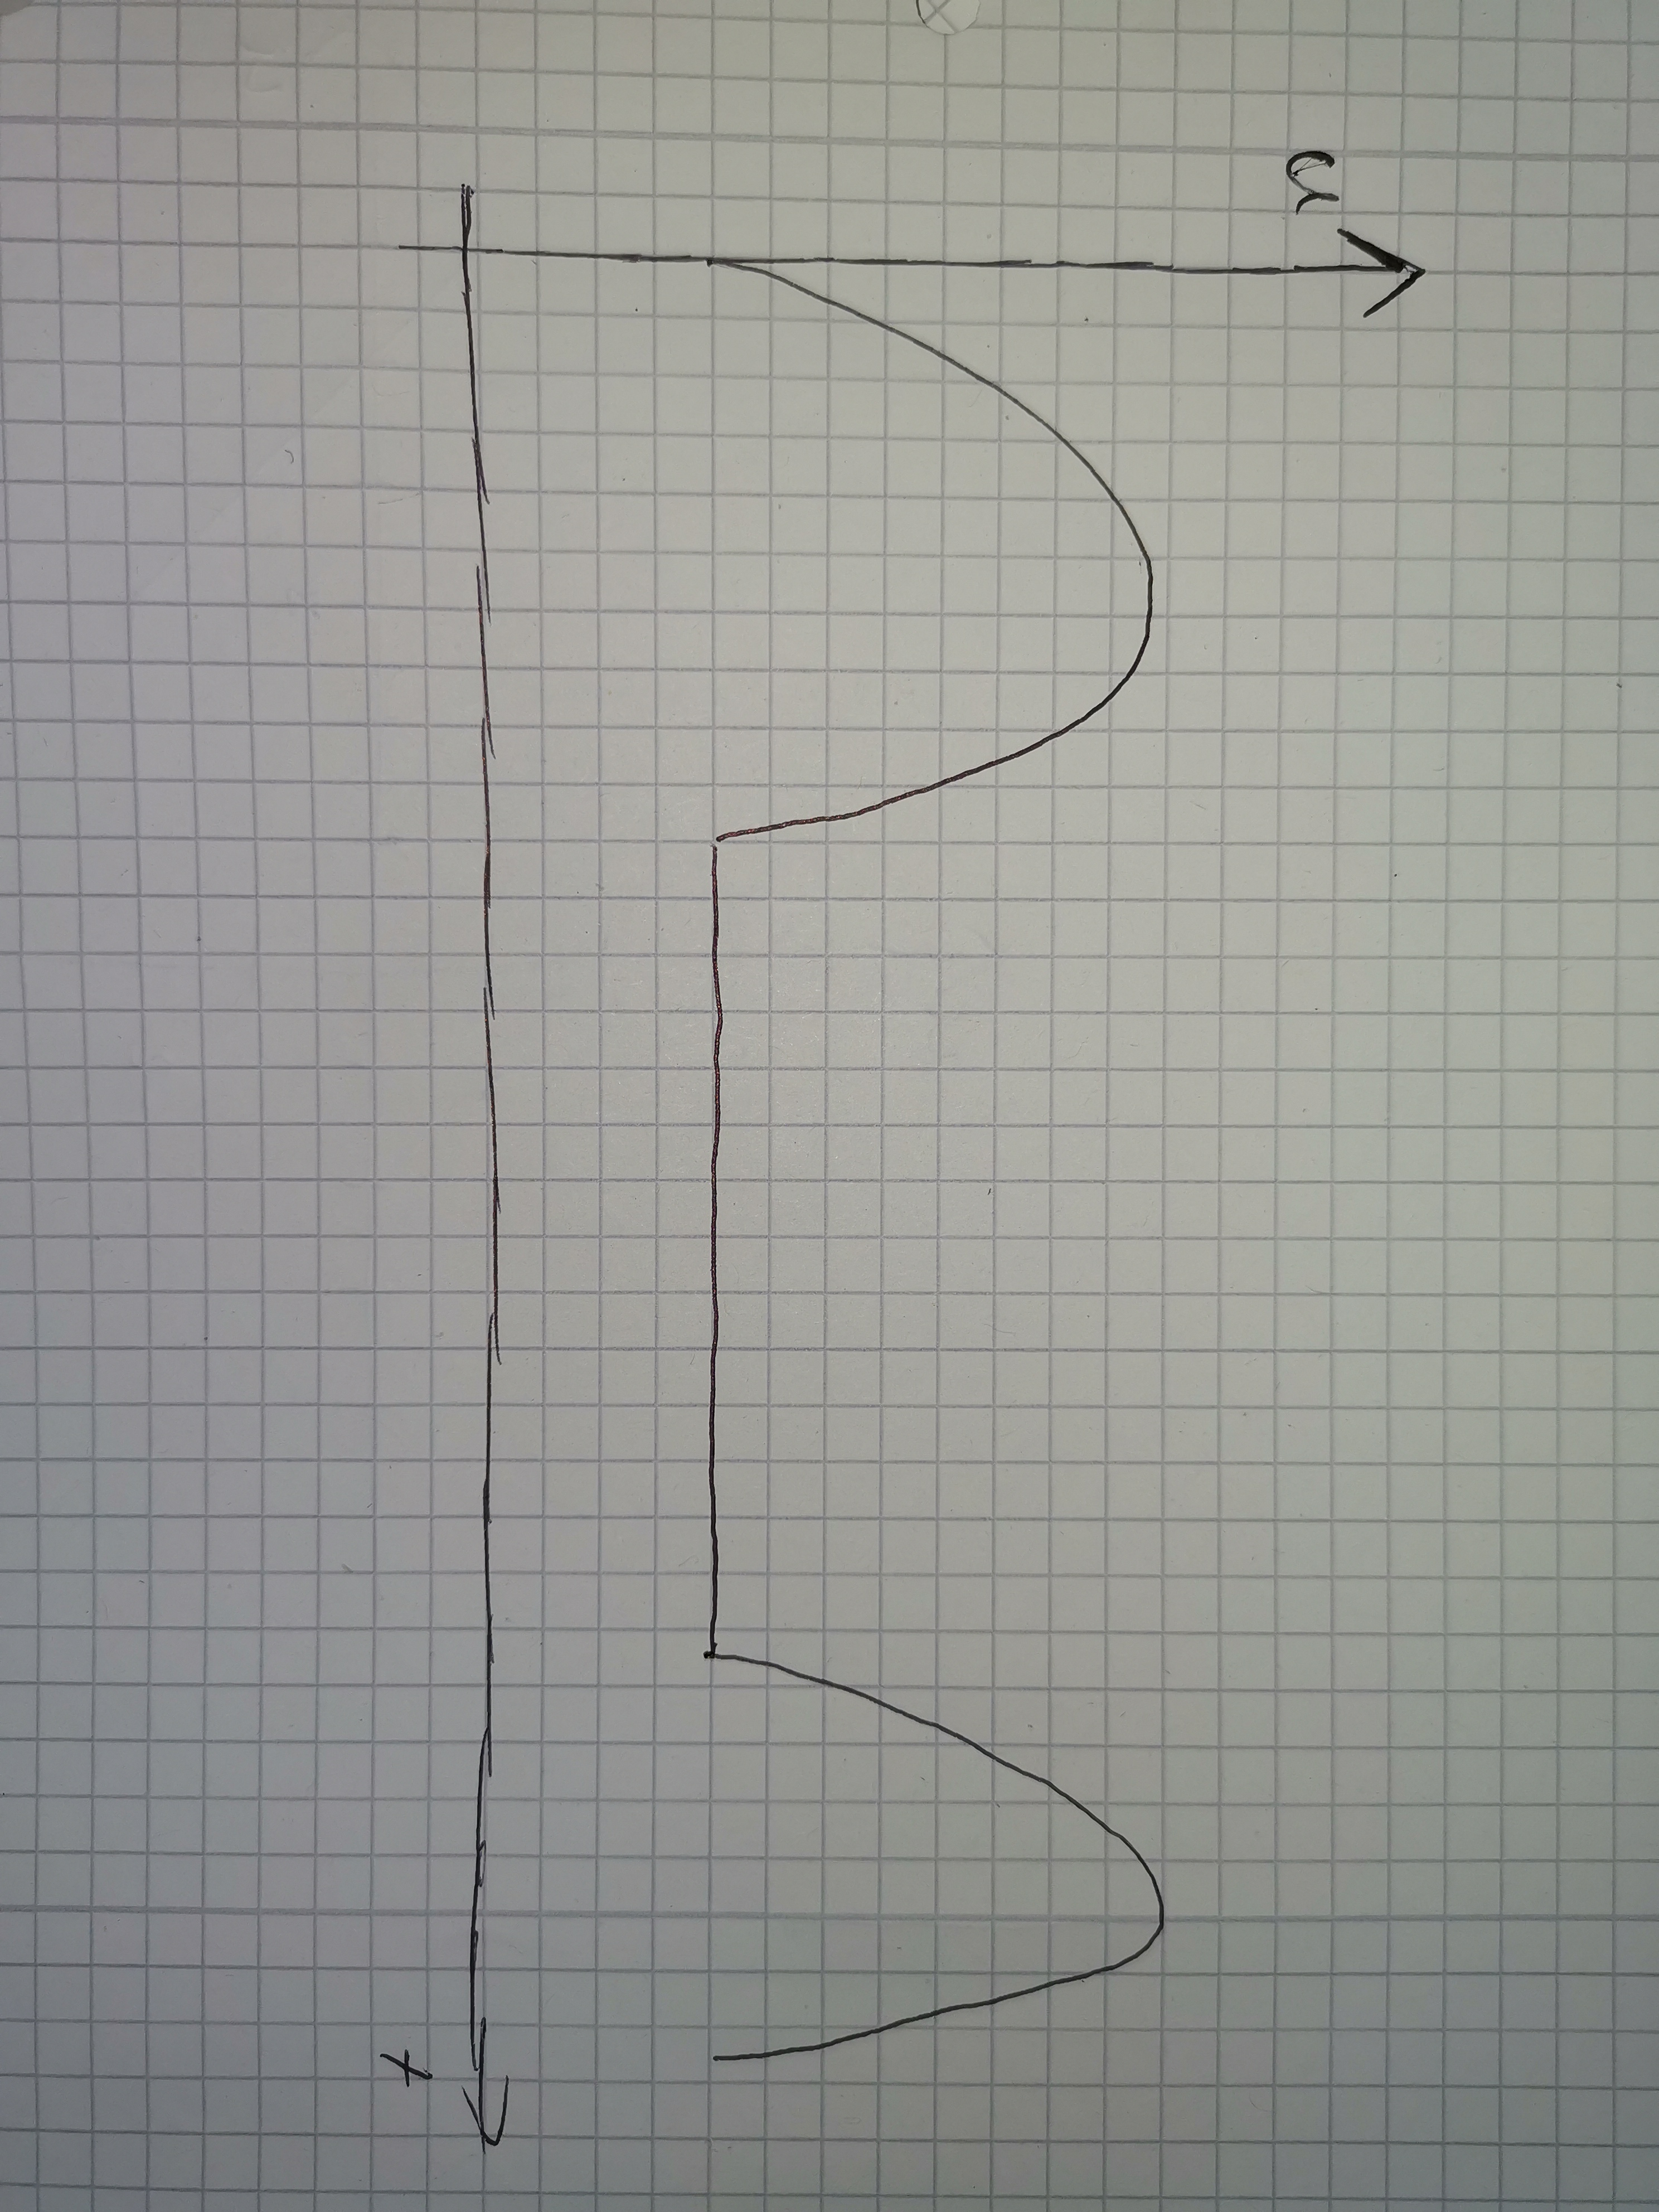
\includegraphics[scale=0.1]{5.jpg}\\
\small \textsc{Abbildung 7 - Skizze Versuch 5}\\
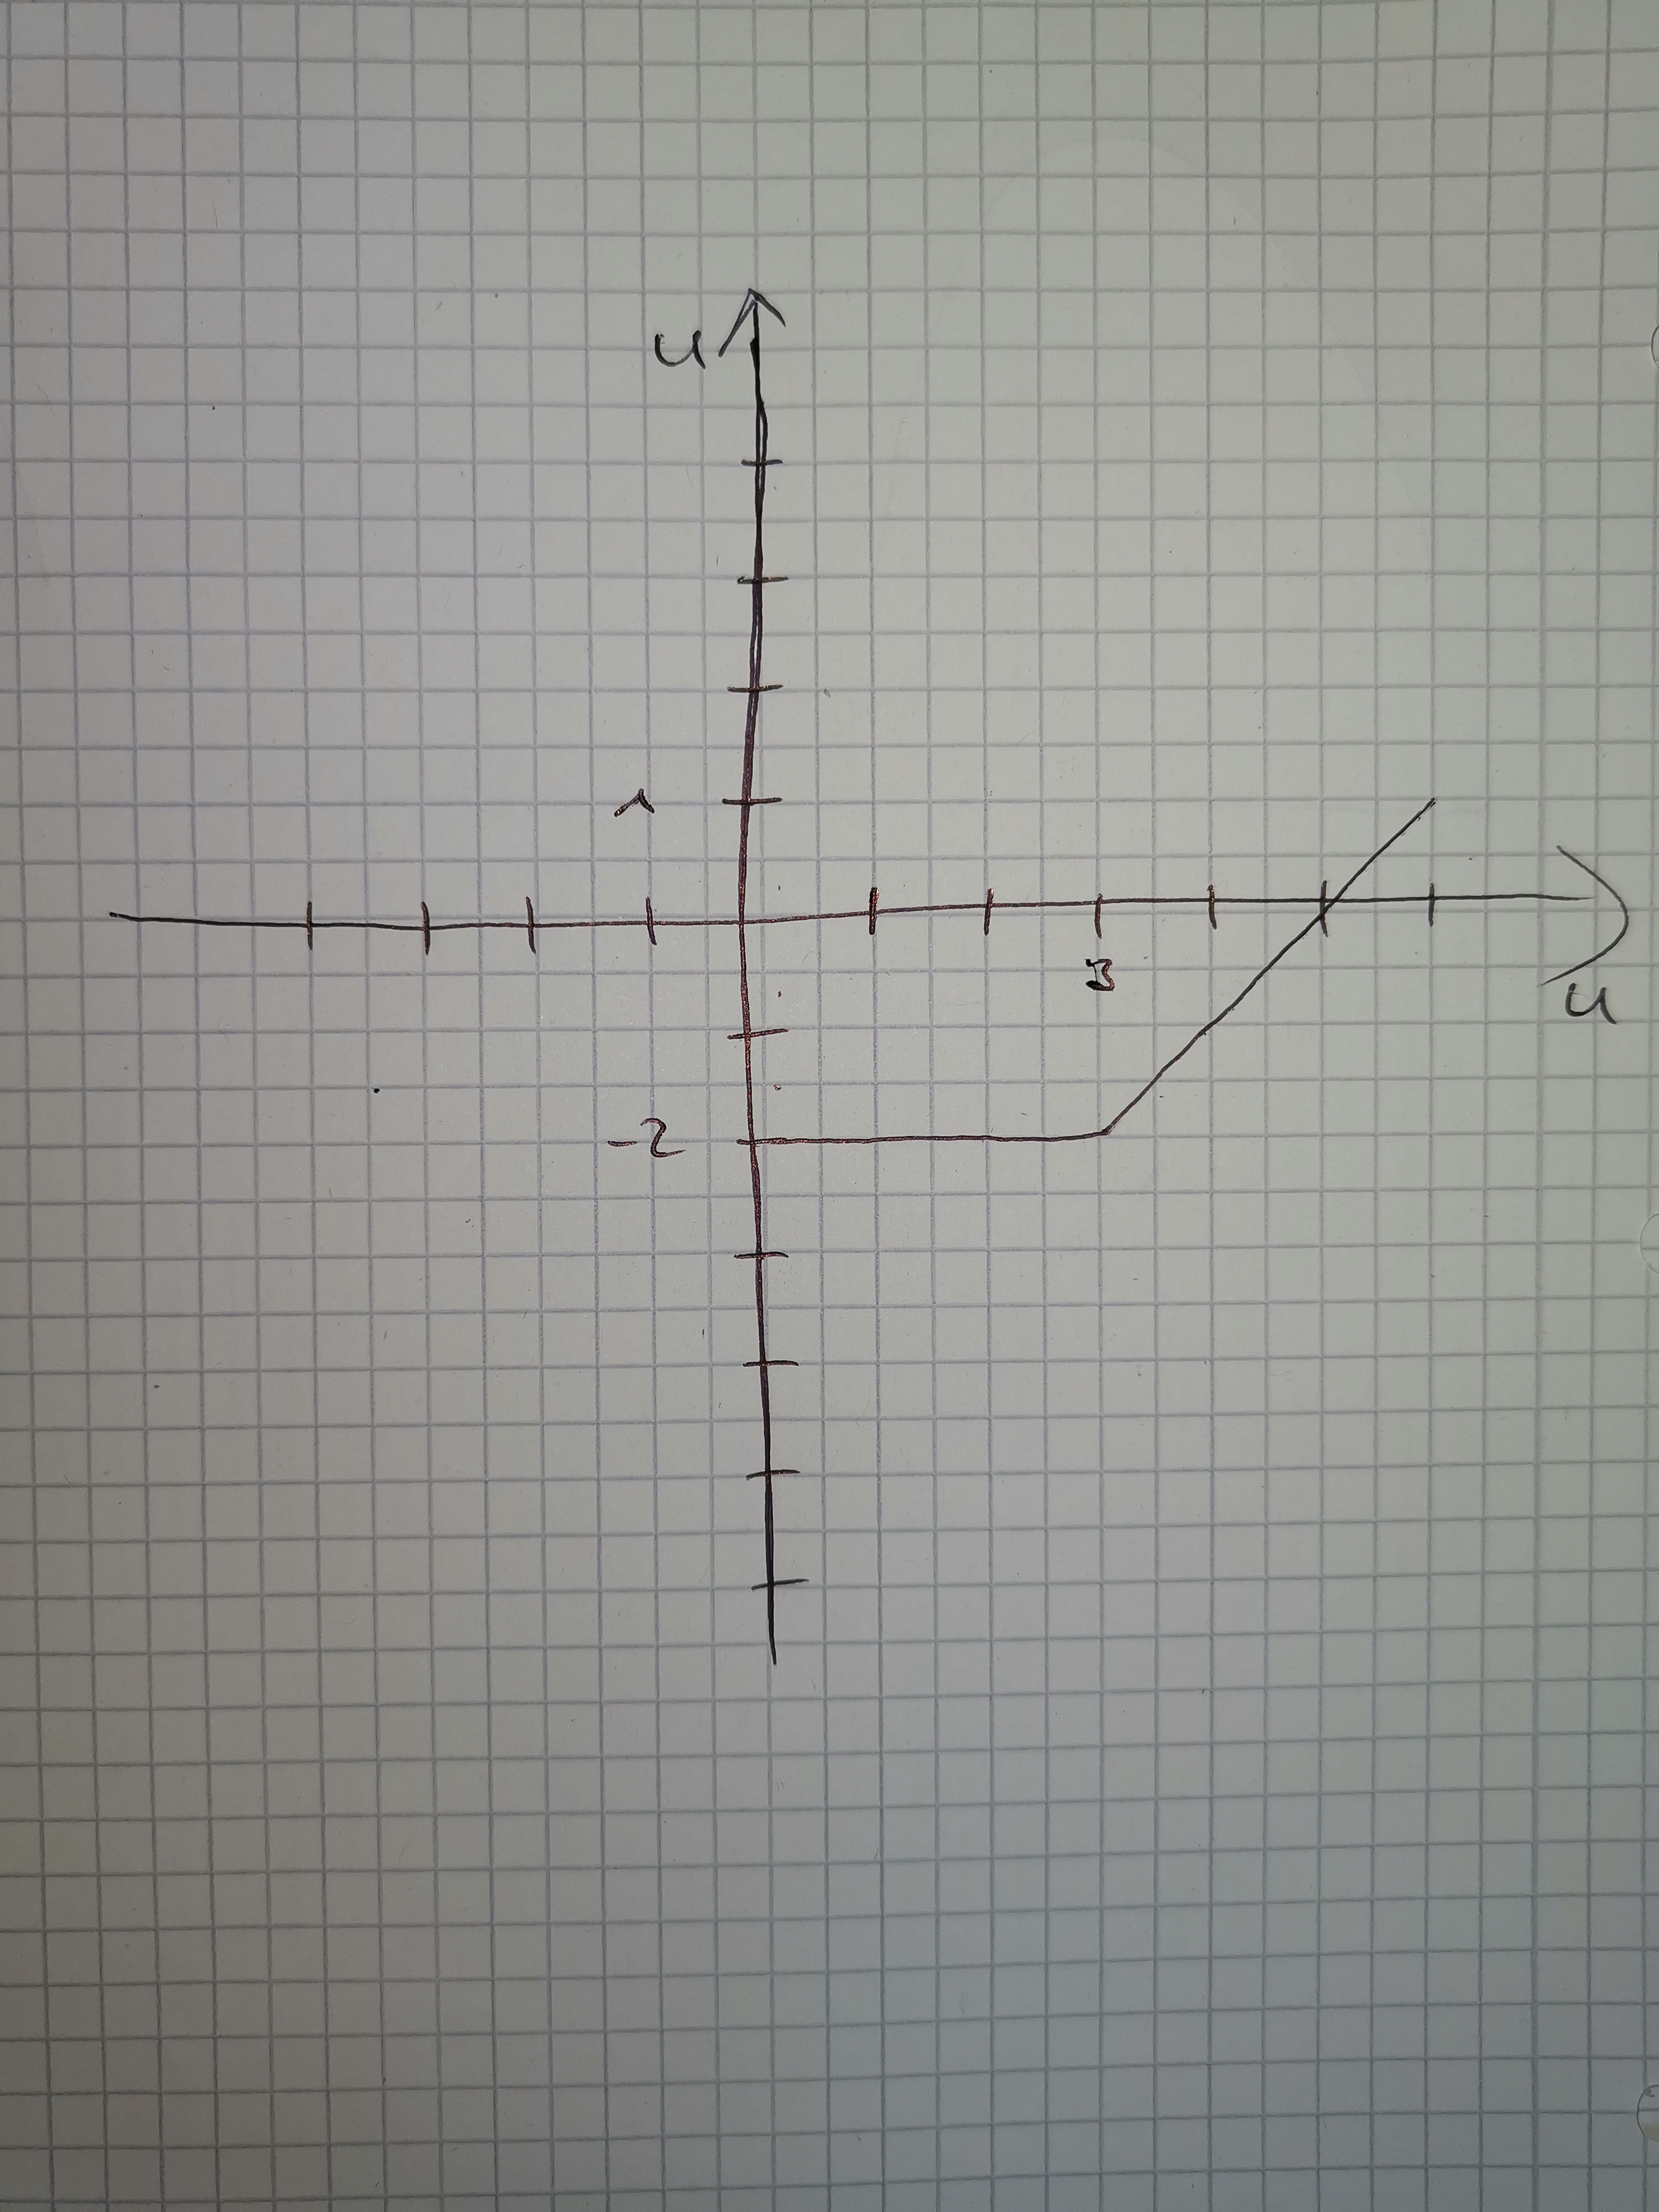
\includegraphics[scale=0.1]{6.jpg}\\
\small \textsc{Abbildung 8 - Skizze Versuch 6}\\
\end{center}

\newpage
\section*{5. Anhang}
\begin{center}
\textsc{Tab. 1 - Messdaten der Spannungsrichtigen und Stromrichtigen Messung}\\
\vspace{3mm}
\begin{tabular}{lcc|lcc}
\multicolumn{3}{c}{\textbf{Spannungsrichtige Messung}} & \multicolumn{3}{c}{\textbf{Stromrichtige Messung}}\\
Gesamtstrom & 0,85 A & 0,0085 A & Gesamtstrom & 0,1 A & 0,30 A \\
Gesamtspannung & 9,2 V & 0,13 V & Gesamtspannung & 8,2 V & 0,082 V \\
Spannung R1 (10 k$\Omega$) & 8,36 V & 0,069 V & Strom R1 (10 k$\Omega$) & 0,0092 V & 0,00012 V\\
Spannung R2 (1 k$\Omega$) & 0,842 V & 0,0077 V & Strom R2 (1 k$\Omega$) & 0,00042 V & 3,5E-05 V\\
Spannungsquotient & 9,93 & 0,070 & Stromquotient & 21,79 & 0,00015\\
Summe d. Spannungsabfälle & 9,202 V & 0,070 V & Summe d. Ströme & 0,0096 V & 0,00015 V\\
\hline
Gesamtstrom & 0,0046 A & 4,6E-05 A & Gesamtstrom & 0,019 A & 0,0032 A\\
Gesamtspannung & 9,2 V & 0,13 V & Gesamtspannung & 9,74 V & 0,069 V\\
Spannung R1 (1 k$\Omega$) & 4,63 V & 0,047 V & Strom R1 (1 k$\Omega$) & 0,0096 V & 0,00012 V\\
Spannung R2 (1 k$\Omega$) & 4,59 V& 0,047 V & Strom R2 (1 k$\Omega$) & 0,0095 V & 0,00014 V \\
Widerstandsquotient & 1,01 & 0,089 & Stromquotient & 1,00 & 0,00027\\
Summe d. Spannungsabfälle & 9,22 V & 0,090 V & Summe d. Ströme & 0,019 V & 0,00027 V\\
\end{tabular}
\end{center}
\vspace{5mm}
\begin{center}
\textsc{Tab. 2 - Messdaten der Widerstandsüberprüfung - Stromrichtig}\\
\vspace{3mm}
\begin{tabular}{l|cc|cc|cc}
Widerstand [$\Omega$] & Spannung [V] & Fehler [V] & Strom [A] & Fehler [A] & Widerstand [$\Omega$] & \\
\hline
0,82 & 0,0892 & 0,0065 & 0,1101 & 0,0014212 & 0,81 & \\
100 & 9,74 & 0,069 & 0,0991 & 0,0012892 & 98,28 & \\
100000 & 9,74 & 0,069 & 0,00098 & 2,176E-05 & 9938,78 & \\
20000000 & 9,74 & 0,069 & 1E-06 & 1,012E-06 & 9740000 & \\
\end{tabular}
\vspace{5mm}

\textsc{Tab. 3 - Messdaten der Wiederstandüberprüfung - Spannungsrichtig}\\
\vspace{3mm}
\begin{tabular}{l|cc|cc|cc}
Widerstand [$\Omega$] & Spannung [V] & Fehler [V] & Strom [A] & Fehler [A] & Widerstand [$\Omega$] & Fehler [$\Omega$]\\
\hline
0,82 & 0,097 & 0,0025 & 0,115 & 0,00238 & 0,84 & 0\\
100 & 9,28 & 0,066 & 0,095 & 0,00214 & 97,68 & 0,07\\
100000 & 9,4 & 0,25 & 0 & 0 & 0 & 0,27\\
20000000 & 9,39 & 0,067 & 0 & 0 & 0 & 20\\
\end{tabular}
\vspace{5mm}

\textsc{Tab. 4 - Messdaten des Versuchs Vier}\\
\vspace{3mm}
\begin{tabular}{l|cccccc}
 Frequenz [Hz] & Spannung [V] & Amplitude [V] & Spitze-Spitze [V] & Effektivwert [V] & Periodendauer [s]\\
1 & 0,3 – 1,3 & 2,5 & 5 & 1,7678 & 1\\
10 & 1,765 & 2,5 & 5 & 1,7678 & 0,1\\
100 & 1,765 & 2,5 & 5 & 1,7678 & 0,01\\
1000 & 1,765 & 2,5 & 5 & 1,7678 & 0,001\\
10000 & 1,065 – 1,069 & 2,5 & 5 & 1,7678 & 0,0001\\
100000 & 0,33 – 0,59 & 2,5 & 5 & 1,7678 & 1E-05\\
\end{tabular}
\end{center}
\end{document}